% from https://topanswers.xyz/tex?q=533#a583
% !TeX TS-program = txs:///duck | convert -delay 60 -loop 0 -density 100 -alpha remove %.pdf %.gif
\documentclass{beamer}
\setbeamertemplate{navigation symbols}{}
\usepackage{tikzlings}
\usetikzlibrary{overlay-beamer-styles}
\setbeamercolor{background canvas}{bg=}
\begin{document}

\begin{frame}

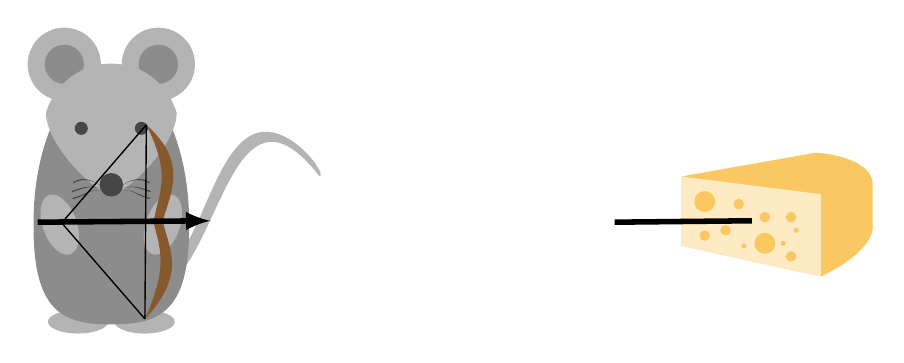
\begin{tikzpicture}[scale=1.66]
  \mouse
  \thing[cheese,xshift=5cm,scale=2,yshift=-0.15cm]
  
  \begin{scope}[yshift=-2.3cm,xshift=-1.4cm,scale=0.7]
  
    % bow
    \path[fill=brown!70!black] (2.3671,3.6028) .. controls (2.8360,4.0984) and (2.6217,4.3820) .. (2.5614,4.6753) .. controls (2.6693,5.0301) and (2.8249,5.3243) .. (2.3827,5.7245) .. controls (2.6589,5.1687) and (2.5253,5.0156) .. (2.4604,4.6598) .. controls (2.5432,4.3450) and (2.6150,4.1629) .. (2.3671,3.6028) -- cycle;
  
    % arrow
    \path<1>[draw=black,line width=2pt,-latex] (1.1936,4.6598) -- (3.0821,4.6753);
    \path<2>[draw=black,line width=2pt] (7.5,4.6598) -- (9,4.6753);

    % bowstring
    \path<1>[draw=black,line width=0.5pt] (2.3671,3.6028) -- (1.4578,4.6520) -- (2.3827,5.7245);
    \path<2>[draw=black,line width=0.5pt] (2.3671,3.6028) -- (2.3827,5.7245);
    
  \end{scope}
  
\end{tikzpicture}
\end{frame}

\end{document}